\documentclass{article}
\usepackage{graphicx}
\usepackage{amsmath}
\usepackage{color}
\usepackage{subcaption}
\usepackage{afterpage}
\usepackage{comment}

\setlength{\oddsidemargin}{10pt}
\usepackage{geometry}
\geometry{letterpaper, portrait, margin=1in}
\title{CSCI-GA 2580 Final Project\\
Query Suggestions and Instant Search Based on Wikipedia Corpus}
\author{Kentaro Hanaki \and Yu-Chih Yu \and Shuang Zhou}

\begin{document}
\maketitle

\section{Introduction}
As search engines are playing an increasingly important role, the expectations of search engines also increase. The historic purpose of search engines is finding relevant documents on the Internet, but nowadays this is far from enough.

Many advanced features are being incorporated into search engines, among which there are two interesting ones: query suggestion and instant search \cite{sigir}. Query suggestion is useful in two ways: First, users do not have to input the entire query and can choose from suggestions. Second, suggestions can provide a general idea about what users want to search when they are not sure.

Instant search perfectly complements query suggestion. With instant search, users can not only see the suggested ``query'', but also searching results, which allow users to be informed of what they are looking for, and thus allow them to refine their query based on retrieved results. Using this two techniques, we provide a more interactive search engine. And with rapid feedback, users can organize their queries more accurately and get more precise results.

This project implements a search engine that adopt this new interaction mode. In the indexing time, our search engine mines the Wikipedia corpus provided in the course assignments and store words and frequencies into Trie and the frequency of n-grams into suffix tree. In the serve time, it also accumulates the users' queries into Trie. For any partial query (prefix or words), our search engine finds most likely completion from the mined data and then recommends a list of relevant queries to users' input.
Meanwhile, the results for the most probable query from the recommendation list along with document snippets are served instantly\footnote{Instant search is first used in Google, and now adopted by some other popular search engines (e.g. Baidu). A lot of our instant search design is inspired by Google.}. All interactions are Ajax-based and no static elements are updated for queries, therefore, the traffic is minimized.

\section{Design and Architecture}

The architecture of our search engine is given in Figure \ref{fig:WorkFlow.png}. We separated the query suggestion into three parts --- word (unigram) suggestion, phrase (n-gram) suggestion and suggestion based on user log. Our initial thought was to store every suffix of the sentences in the corpus to the suffix trie because we do not have query log history, the entire corpus would be a good source for us to give suggestion. But storing the entire corpus not only runs longer to index and load but also uses a lot more memory. Therefore, we decided to separate the corpus-based suggestion into word suggestion and phrase suggestion.

The first part is word suggestion. When a user types some word prefix, the search engine suggests words that share the same prefix with the order of frequencies in the corpus. Our assumption is that the more frequent the word is, the more likely the user wants to start to search with the word. Ideally, the ranking should be done based on frequencies in query logs, but we would expect that corpus frequency is an approximation of query log frequency.

The second part is phrase suggestion. In order to reduce the size of the suggestion data structure, we decided not to use suffix trie \cite{intro}. Alternatively, we treat each word as a smallest unit in the data structure, i.e., representing each word with a number. So a sentence will become a short sequence of numbers instead of a long sequence of letters and spaces. These sequence can be put into the suffix tree. But putting all suffix numbers of a sentence is not efficient enough, so instead of putting every suffix, we set a maximum length of the suffix to 3, simply because setting it to 2 did not work well and setting it to 4 uses too much memory. Finally we reduced the size of the tree by pruning branches that are not frequent (100 times for single word, 10 times for bigram and 5 times for trigram).

The thrid part is user logged suggestion. It is similar to the first part except that it stores all the user queries into Trie instead of only a single word from the dictionary.

\begin{figure}
\centering
\setlength\fboxrule{0.5pt}
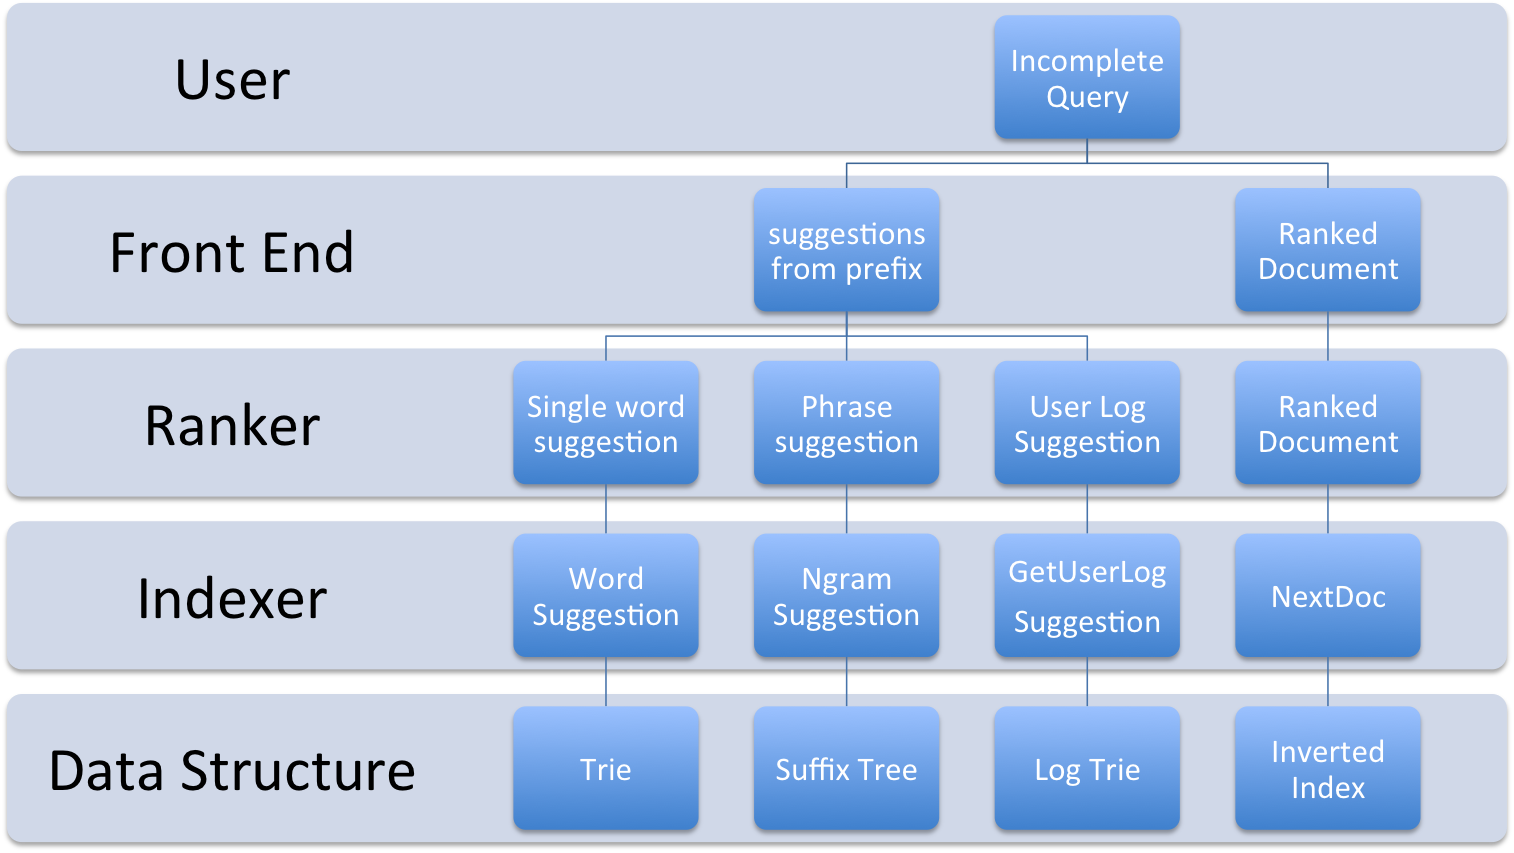
\includegraphics[scale=0.6] {WorkFlow.png}
\caption{This is the flow diagram of our project. Example: when user types "Google", it will get ["google map", "google translate"...] and also the instant search result from front end. And then front end gets result from ranker and then indexer and finally interact with our data structure.}
\label{fig:WorkFlow.png}
\end{figure}

\section{Implementation Details}

In this section, we briefly go over our implementations. The instruction about how to run the program is given in read me.txt in our repository. 
\begin{enumerate}
  \item Single word suggestion
  \begin{itemize}
  \item  Indexing: store every word from the data set in a single Trie with their frequencies.
  \item Suggestion: return all words that the prefix match the query along with the frequencies. 
  \item Ranking: return the words with top 8 frequencies.
\end{itemize}
	
	
  \item Phrase suggestion
  
  \begin{itemize} 
	\item Indexing: store uni-gram, bi-gram, and tri-gram of all adjacent words from the data set into a suffix tree.
	\item Suggestion: return all N-grams that the prefix match the query along with frequencies.
	\item Ranking: return the N-grams with top 8 frequencies.
\end{itemize}
  \item Logged query suggestion
  \begin{itemize} 

\item Indexing: store the whole query issued by the user including the space in a trie along with their frequencies.
\item Suggestion: return all queries that the prefix match the query along with their frequencies.
\item Ranking: return the queries with up to top 4 frequencies.
\end{itemize}

\item

Merge the suggestions from the above three components and return 8 results to front end.

\item

Front end put an event listener on the input box, and request suggestions whenever the event is triggered (e.g. user stops typing), then the page instantly load the results of the most likely query.
	

\end{enumerate}

%readme should be copied from here
\begin{comment}
Step  1: unzip source.zip
Step  2: cd source
Step  3: Then compile code
	javac -cp lib/jsoup-1.8.1.jar src/edu/nyu/cs/cs2580/*.java
Step  4: Build index before running the server
	java -cp src:lib/jsoup-1.8.1.jar -Xmx4G edu.nyu.cs.cs2580.SearchEngine --mode=index --options=conf/engine.conf
Step  5: To start to server listening at port 25813
	java -cp src:lib/jsoup-1.8.1.jar -Xmx4G  edu.nyu.cs.cs2580.SearchEngine --mode=serve --options=conf/engine.conf --port=25813
Step 6: Alternatively, step 3 through 5 can be combined using a single command
	./run.sh or sh run.sh
Step 7: Open web/home.html to start enjoying our search engine
\end{comment}
		

\section{Evaluation}

In this section, we evaluate our query suggestion algorithms. The goal of our project is to approximate the query suggestions based on query logs using information from corpus. Therefore, we compare the results of our algorithm to the suggestions from the commercial web search engine. More specifically, we compare our result to the results from Google. 

We examined the quality of completion in the following cases:
\begin{itemize}
\item The first case is when the first three characters of words are typed. Our search engine suggest single words in this case.
\item The second case is when one or two words are typed. Our search engine suggests phrases based on the words entered.
\end{itemize}
In both cases, we compared the results with Google suggestions. More specifically, we took top $4$ suggestions from both our search engine and Google and see if those suggestions agree. In order to avoid unnecessary personalization, we conducted the experiment after logging out from Google account. Also, our search engine can suggest previously searched queries, but we turned off this functionality.

\begin{figure}[!h]
\begin{center}
\begin{tabular}{| l | l | l | l |}
\hline
Prefix & Our system suggestions & Google suggestions & Accuracy \\
\hline
alg- & algebraic & algebra & 0.5 \\
& algorithms & algebra calculator & \\
& {\bf \color{red} algorithm} & {\bf \color{red} algorithm} & \\
& {\bf \color{red} algeria} & {\bf \color{red} algeria} & \\
\hline
pra- & practice & prada & 0\\
& practices & prankdial & \\
& practical & pratt institute & \\
& praised & practice fusion & \\
\hline
\end{tabular}
\end{center}
\caption{Results of suggestions from prefix. Bold red suggestions are the ones that show up both in our search engine and in Google.}
\label{fig:word}
\end{figure}

Figure \ref{fig:word} shows the suggestions for two example prefixes (`alg-' and `pra-'). `alg-' achieved the accuracy of $0.5$, and different suggestions are also similar (`algebraic' and `algebra'). On the other hand, our system suggestions for `pra-' are too general and differ a lot from Google's results. This stems from the fact that our suggestions are based purely on frequencies in Wikipedia corpus and not on query logs. Thus it can suggest words that appears frequently in English texts but are not searched by users.

\begin{figure}[!h]
\begin{center}
\begin{tabular}{| l | l | l | l |}
\hline
Word & Our system suggestions & Google suggestions & Accuracy \\
\hline
political & {\bf \color{red} political parties} & political cartoons & 0.5 \\
& {\bf \color{red} political science} & {\bf \color{red} political science} & \\
& political hip hop & political compass & \\
& political economy & {\bf \color{red} political parties} & \\
\hline
new & new york & {\bf \color{red} new york times} & 0.25\\
& {\bf \color{red} new york times} & new york lottery & \\
& new york city & new york post & \\
& new zealand & new jersey transit & \\
\hline
michigan & michigan press & michigan  & 0 \\
& michigan minnesota mississippi & michigan football & \\
& michigan state university & michigan state football & \\
& michigan state & michigan football schedule & \\
\hline
\end{tabular}
\end{center}
\caption{Results of phrase suggestions. Bold red suggestions are the ones that show up both in our search engine and in Google.}
\label{fig:phrase}
\end{figure}

Figure \ref{fig:phrase} shows the results for phrase suggestions. First of all, most of the suggested phrases in the experiment make sense, although there are some phrases that do not make sense (`michigan minnesota mississippi', which came from the list of states). Among the words we experimented, `political' achieved $0.5$ accuracy (`political parties' and `political science' agreed). Accuracy for `new' was $0.25$, and disagreement stems from the fact that Google uses location information (we searched from NYU and got `new jersey transit'). 

Finally, there is an interesting difference in the suggestions for `michigan'. Our search engine suggested press and university, although Google suggested phrases related to football. This is because Google uses query logs to improve the suggestions. Most of American people are interested college football for Michigan rather than press or university itself, and this interest is reflected on the suggestions by Google.


\section{Contributions}

\begin{itemize}
\item Kentaro Hanaki: He was responsible for ranking and evaluating suggestions. He implemented the ranking procedure and designed/conducted the evaluation for suggestions. He also implemented logging of user queries.
\item Calvin Yu: He was responsible for data structures for query suggestions. He designed and implemented efficient data structures for building and scoring suggestions from query prefix/words.
\item Shuang Zhou: He was primarily responsible for front end. More specifically, he designed graphic user interface, designed and implemented asynchronous request to the server using Ajax, and implemented snippets.
\end{itemize}


\begin{thebibliography}{1}

\bibitem{sigir} H. Bast and I. Weber. Type less, find more: fast autocompletion search with a succinct index. In {\em SIGIR}, pages 364-€“371, 2006.
\bibitem{intro} T. H. Cormen, C. E. Leiserson, R. L. Rivest and C. Stein. {\em Introduction to Algorithms, third edition}, June 2007.

\end{thebibliography}

\end{document}
